\documentclass[tikz,border=10pt]{standalone}
\usepackage{tikz}
\usetikzlibrary{arrows.meta, positioning}

\begin{document}

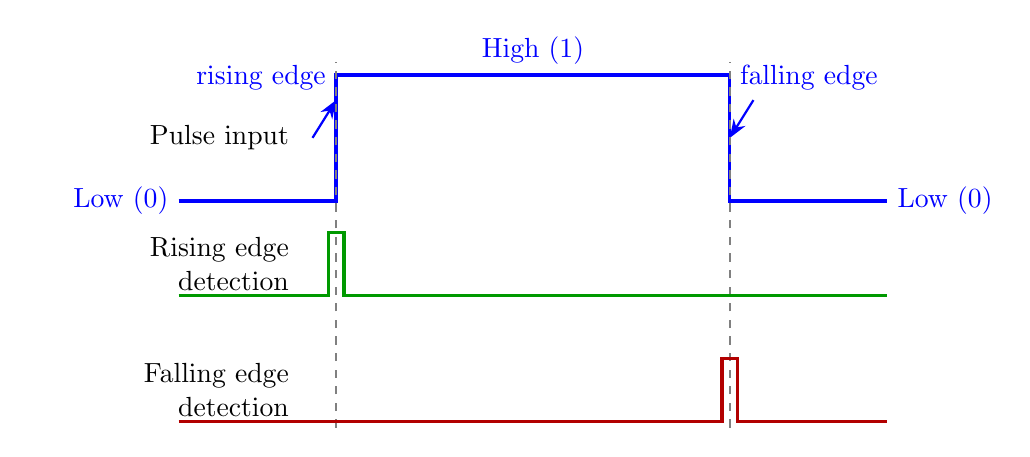
\begin{tikzpicture}[
    x=1cm,
    y=0.8cm,
    >=Stealth,
    thick,
    signal/.style={line width=1.2pt},
    label/.style={align=right, text width=3.2cm}
]

% Time markers
\def\tA{2}
\def\tB{7}
\def\tC{9}

% =========================
% Pulse input
% =========================
\node[label] at (-0.2,4) {Pulse input};

\draw[signal, blue]
    (0,3) -- (\tA,3)
    -- (\tA,5)
    -- (\tB,5)
    -- (\tB,3)
    -- (\tC,3);

% Logic labels
\node[blue, above] at (4.5,5) {High (1)};
\node[blue, left]  at (0,3) {Low (0)};
\node[blue, right] at (\tC,3) {Low (0)};

% Rising / Falling edge arrows
\draw[->, blue] (\tA-0.3,4) -- (\tA,4.6);
\node[blue, above left] at (\tA,4.6) {rising edge};

\draw[->, blue] (\tB+0.3,4.6) -- (\tB,4);
\node[blue, above right] at (\tB,4.6) {falling edge};

% Timing markers
\draw[dashed, gray] (\tA,-0.6) -- (\tA,5.2);
\draw[dashed, gray] (\tB,-0.6) -- (\tB,5.2);

% =========================
% Rising edge detection output
% =========================
\node[label] at (-0.2,2) {Rising edge\\detection};

\draw[signal, green!60!black]
    (0,1.5) -- (\tA-0.1,1.5)
    -- (\tA-0.1,2.5)
    -- (\tA+0.1,2.5)
    -- (\tA+0.1,1.5)
    -- (\tC,1.5);

% =========================
% Falling edge detection output
% =========================
\node[label] at (-0.2,0) {Falling edge\\detection};

\draw[signal, red!70!black]
    (0,-0.5) -- (\tB-0.1,-0.5)
    -- (\tB-0.1,0.5)
    -- (\tB+0.1,0.5)
    -- (\tB+0.1,-0.5)
    -- (\tC,-0.5);

\end{tikzpicture}

\end{document}
